\providecommand{\itescastudentname}{Martin Jonathan de la Cruz}
\providecommand{\itescastudentshort}{M. J. de la Cruz}
\providecommand{\itescastudentid}{ITESCA-MGA}
\providecommand{\itescafaculty}{Instituto Tecnologico Superior de Cajeme}
\providecommand{\itescafacultyname}{Maestria en Gestion Administrativa}
\providecommand{\itescacoursename}{Analisis y Desarrollo Economico}
\providecommand{\itescacoursecode}{MGA-ANALISIS-Y-DESARROLLO-ECONOMICO}
\providecommand{\itescadepartment}{Analisis y Desarrollo Economico}
\providecommand{\itescateachingfigure}{Docente de la materia por definir}
\providecommand{\itescaprogramlevel}{Maestria}
\providecommand{\itescaprogramperiod}{Periodo academico por definir}
\providecommand{\itescamodality}{Modalidad por definir}
\providecommand{\itescaprofessionalprofile}{La Maestria en Gestion Administrativa exige analizar decisiones organizacionales con criterio, evidencia, pertinencia institucional y enfoque de mejora.}
\providecommand{\itescatransfercontext}{Analisis y Desarrollo Economico, contexto profesional y aplicacion disciplinar}
\providecommand{\itescalocation}{Cajeme, Sonora}
\providecommand{\itescalocationname}{Cajeme, Sonora}
\providecommand{\itescabibliography}{bibliografia-itesca-mga,ITESCA/maestria-en-gestion-administrativa/analisis-y-desarrollo-economico-mga/analisis-y-desarrollo-economico}
\providecommand{\itescageneralbib}{bibliografia-itesca-mga.bib}
\providecommand{\itescacoursebib}{analisis-y-desarrollo-economico.bib}

\providecommand{\itescamethodologycore}{Problema -> diagnostico -> evidencia -> decision -> consecuencia -> mejora}
\providecommand{\itescawritingmodel}{Redaccion critica, argumentacion ejecutiva y analisis profundo orientado a gestion}
\providecommand{\itescadidactictechniques}{Estudio de caso, matriz de priorizacion, cuadro comparativo, ensayo critico, debate, portafolio y proyecto integrador}

\def\itescadocumenttitle {Analisis y Desarrollo Economico}
\def\itescadocumentsubtitle {Contenedor base de materia}
\def\itescadocumentsubject {Analisis y Desarrollo Economico}
\def\itescaactivityname {Punto de entrada canonico de materia}
\def\itescasessionname {Analisis y Desarrollo Economico}
\def\itescablockname {tronco comun MGA}
\def\itescamainproduct {Informe academico base de la materia}

% ==============================================================================
% PLANTILLA MAESTRA GENERAL - ITESCA
% ============================================================================== 
% Uso:
% 1. Duplica el archivo contenedor de la materia o actividad y actualiza sus
%    metadatos editables.
% 2. Conserva el enfoque de trabajo: no pegar instrucciones completas dentro del
%    documento final; usar la planeacion como lista de cumplimiento.
% 3. Construye productos visuales en LaTeX/TikZ cuando la actividad lo pida.
% 4. Mantiene citas autor-anio con natbib y bibliografia en BibTeX.
% 5. Cierra con criterio propio, no con un resumen plano.
%
% Formato institucional recomendado para ITESCA:
% - Fuente sans serif tipo Helvetica.
% - Interlineado 1.5.
% - Portada institucional, abstract, desarrollo, postura y conclusion.
% - Citas autor-anio con natbib: usar \citep{clave} o \citet{clave}.
% - Bibliografia en BibTeX, consistente con el producto real.
% - Comentarios operativos dentro del archivo para sostener la redaccion.
% - Identidad institucional visible mediante logotipo oficial, marca de agua y
%   vinculacion con la carrera o el contexto profesional.
%
% Criterios generales de cumplimiento:
% - Responder exactamente a la actividad solicitada por la materia o docente.
% - Convertir la consigna en problema, analisis, evidencia y consecuencia.
% - Relacionar el tema con la carrera, la materia y el contexto institucional.
% - Analizar, interpretar y tomar postura; no solo recopilar definiciones.
% - Mostrar producto visible cuando la actividad pida cuadro, esquema, tabla,
%   mapa, diagrama, evidencia o procedimiento.
% - Cerrar con criterio propio, aprendizaje y aplicacion transferible.
%
% Regla para productos visuales:
% - Si la actividad pide cuadro comparativo, mapa, linea de tiempo, matriz,
%   tabla, diagrama o evidencia analitica, construirlo preferentemente en
%   LaTeX/TikZ para mantener nitidez, control y edicion futura.
% - Si la actividad exige herramienta externa, insertar una imagen nitida y
%   conservar la explicacion dentro del documento.
%
% Criterios de redaccion personal:
% - No escribir para llenar espacio; escribir para sostener una idea.
% - Convertir informacion en criterio: que significa, como funciona, que limite
%   presenta, que riesgo aparece y que consecuencia produce.
% - Formula util: concepto -> funcion -> problema -> consecuencia -> postura.
% - La postura personal no debe ser opinion suelta. Debe tener posicion, razon y efecto.
% - La conclusion no debe repetir el desarrollo: debe sintetizar y proyectar.
%
% Control editorial ITESCA:
% - Cada actividad debe tener una ficha de lectura: consigna, producto,
%   evidencia, criterio de evaluacion y transferencia profesional.
% - La identidad institucional no debe limitarse al logotipo. Debe aparecer en
%   la forma de argumentar: precision tecnica, pertinencia academica,
%   vinculacion con carrera y utilidad profesional.
% - Evitar la respuesta generica. El documento debe mostrar que problema atiende
%   la actividad, que decision metodologica se tomo y que evidencia permite
%   sostener el resultado.
% - Cuando la actividad sea de induccion, diagnostico o primer ingreso, traducir
%   el contenido a habitos universitarios: lectura, organizacion, evidencia,
%   integridad academica, autonomia y seguimiento institucional.
% - Cuando la actividad sea disciplinar, traducir el contenido a un proceso,
%   sistema, caso, herramienta, decision administrativa, tecnica o profesional.
%
% Regla de nivel minimo:
% - Si la actividad solo pide identificar o describir, elevar el producto a
%   comprension aplicada: explicar funcion, limite y ejemplo.
% - Si pide cuadro, mapa, matriz, evidencia o conclusion, llegar por lo menos a
%   analisis: comparar criterios, justificar diferencias y cerrar con postura.
% - Si pide propuesta, procedimiento o solucion, llegar a evaluacion/creacion:
%   definir criterios, construir producto propio y justificar su pertinencia.
%
% Voz editorial esperada:
% - Academica, directa, institucional y funcional.
% - No sonar como copia de fuentes ni como resumen escolar.
% - Usar criterio personal con moderacion: posicion, razon y efecto.
% - Antes de redactar, decidir la funcion de cada seccion: abrir problema,
%   delimitar criterio, demostrar con evidencia, valorar o concluir.
%
% Nivel cognitivo esperado:
% - Comprender: explicar el tema con lenguaje propio.
% - Aplicar: llevar el concepto a un caso, proceso, procedimiento o producto.
% - Analizar: distinguir componentes, tensiones, limites y decisiones.
% - Evaluar: sostener un criterio con razones y consecuencias.
% - Crear: construir un producto propio cuando la actividad lo solicite.
%
% Checklist antes de entregar:
% [ ] Titulo, actividad, asignatura, codigo, docente y fecha actualizados.
% [ ] Tecnica didactica identificada y justificada.
% [ ] Existe una tesis, postura o criterio central.
% [ ] La evidencia permite sostener las conclusiones.
% [ ] Se demuestra transferencia academica o profesional.
% [ ] El objetivo coincide con la consigna real.
% [ ] El producto solicitado aparece visible y completo.
% [ ] La introduccion plantea un problema y no solo anuncia el tema.
% [ ] El desarrollo explica, conecta y analiza.
% [ ] El texto aterriza el tema a la carrera o al contexto profesional.
% [ ] Hay citas autor-anio y bibliografia consistente.
% [ ] La conclusion responde que se comprendio y que criterio se sostiene.
% [ ] Quitar o comentar \pendiente cuando el documento final este terminado.
% ============================================================================== 

% ------------------------------------------------------------------------------
% METADATOS EDITABLES
% ------------------------------------------------------------------------------
\providecommand{\itescadocumenttitle}{Plantilla institucional ITESCA}
\providecommand{\itescadocumentsubtitle}{Actividad X}
\providecommand{\itescadocumentsubject}{Informe academico}
\providecommand{\itescastudentname}{Martin Jonathan de la Cruz}
\providecommand{\itescastudentid}{ITESCA}
\providecommand{\itescacoursename}{Nombre de la asignatura}
\providecommand{\itescacoursecode}{ITESCA}
\providecommand{\itescafaculty}{Programa academico ITESCA}
\providecommand{\itescadepartment}{Departamento academico}
\providecommand{\itescateachingfigure}{Nombre por definir}
\providecommand{\itescastudentemail}{correo.institucional@itesca.edu.mx}
\providecommand{\itescaprogramlevel}{Nivel academico por definir}
\providecommand{\itescaprogramperiod}{Periodo academico por definir}
\providecommand{\itescamodality}{Modalidad por definir}
\providecommand{\itescaactivityname}{Actividad por definir}
\providecommand{\itescasessionname}{Sesion por definir}
\providecommand{\itescablockname}{Bloque por definir}
\providecommand{\itescamainproduct}{Producto academico por definir}
\providecommand{\itescaprofessionalprofile}{Perfil profesional por definir}
\providecommand{\itescainstitutionalaxis}{Formacion academica, identidad institucional y transferencia profesional}
\providecommand{\itescaevidencefocus}{Evidencia academica, producto visible y criterio propio}
\providecommand{\itescaqualitycriterion}{Claridad, pertinencia, evidencia, analisis y cierre transferible}
\providecommand{\itescatransfercontext}{Carrera, asignatura, entorno profesional o trayectoria formativa}
\providecommand{\itescalocation}{Cajeme, Sonora}
\providecommand{\itescabibliography}{bibliografia-itesca-mga,ITESCA/maestria-en-gestion-administrativa/analisis-y-desarrollo-economico-mga/analisis-y-desarrollo-economico}
\providecommand{\itescaasset}{ITESCA/assets-itesca/itesca-monograma.png}
\providecommand{\itescaofficialasset}{ITESCA/assets-itesca/web/logo-itesca-contorno.png}
\providecommand{\itescasecondaryasset}{ITESCA/assets-itesca/itesca-monograma.png}
\providecommand{\itescacampusurl}{https://www.itesca.edu.mx/}
\providecommand{\itescaportalurl}{https://www.itesca.edu.mx/portalacademico/}
\providecommand{\itescavirtualurl}{https://www.itesca.edu.mx/modulos/oferta/ead/index.php}

% CREACION DEL DOCUMENTO
\documentclass[
	spanish,
	letterpaper, oneside
]{article}

% INFORMACION DEL DOCUMENTO
\def\documenttitle {\itescadocumenttitle}
\def\documentsubtitle {\itescadocumentsubtitle}
\def\documentsubject {\itescadocumentsubject}

\def\documentauthor {\itescastudentname}
\def\coursename {\itescacoursename}
\def\coursecode {\itescacoursecode}

\def\universityname {Instituto Tecnologico Superior de Cajeme}
\def\universityfaculty {\itescafaculty}
\def\universitydepartment {\itescadepartment}
\def\universitydepartmentimage {\itescaofficialasset}
\def\universitydepartmentimagecfg {width=5.2cm}
\def\universitylocation {\itescalocation}

% INTEGRANTES, PROFESORES Y FECHAS
\def\authortable {
	\begin{tabular}{ll}
		\textbf{Alumno:}
		& \begin{tabular}[t]{l}
			 \itescastudentname \\
		\end{tabular} \\
		Matricula: & \itescastudentid \\
		Correo institucional: & \itescastudentemail \\
		Asignatura: & \itescacoursename \\
		Codigo: & \itescacoursecode \\
		Nivel: & \itescaprogramlevel \\
		Periodo: & \itescaprogramperiod \\
		Modalidad: & \itescamodality \\

		\textit{Figura docente:}
		& \begin{tabular}[t]{l}
			\itescateachingfigure
		\end{tabular} \\
		Sesion/Bloque: & \itescasessionname\ / \itescablockname \\
		Producto: & \itescamainproduct \\
		& \\
		\multicolumn{2}{l}{Fecha de realizacion: \today} \\
		\multicolumn{2}{l}{\universitylocation}
	\end{tabular}
}

% IMPORTACION DEL TEMPLATE BASE
\input{template}

% FORMATO GENERAL
\usepackage{helvet}
\renewcommand{\familydefault}{\sfdefault}

% IDENTIDAD VISUAL ITESCA
\definecolor{itescaRedDark}{HTML}{8F1117}
\definecolor{itescaRed}{HTML}{D70F18}
\definecolor{itescaCharcoal}{HTML}{141414}
\definecolor{itescaSilver}{HTML}{D9D9D9}
\definecolor{itescaPaper}{HTML}{F7F7F7}
\definecolor{itescaInk}{HTML}{181818}
\definecolor{itescaMuted}{HTML}{6A6A6A}
\colorlet{itescaGreenDark}{itescaRedDark}
\colorlet{itescaGreen}{itescaCharcoal}
\colorlet{itescaGold}{itescaSilver}
\def\portraittitlecolor {itescaRedDark}

% TABLAS Y PRODUCTOS VISUALES
\usepackage{array}
\usepackage{longtable}
\usepackage{pdflscape}
\usepackage{tikz}
\usetikzlibrary{
	arrows.meta,
	positioning,
	calc,
	matrix,
	fit,
	shapes.geometric,
	shadows.blur
}

% CITAS EN FORMATO AUTOR-ANIO, COMPATIBLE CON APA 7 EN EL CUERPO DEL TEXTO
\setcitestyle{authoryear,open={(},close={)}}

% AYUDAS DE REDACCION
% Quitar o comentar \pendiente cuando el documento final este terminado.
\newcommand{\pendiente}[1]{\textcolor{red}{Refuerzo Ciclo A materializado}}

% MARCA DE AGUA EN PORTADA
\def\coverwatermarkenabled {true}
\def\coverwatermarkimage {\itescaasset}
\def\coverwatermarkopacity {0.13}
\def\coverwatermarkwidth {0.58\paperwidth}
\def\coverwatermarkxshift {0cm}
\def\coverwatermarkyshift {-0.10cm}

\newcommand{\insertcoverwatermark}{%
	\ifthenelse{\equal{\coverwatermarkenabled}{true}}{%
		\AddToShipoutPictureBG*{%
			\begin{tikzpicture}[remember picture,overlay]
				\node[
					opacity=\coverwatermarkopacity,
					inner sep=0pt,
					xshift=\coverwatermarkxshift,
					yshift=\coverwatermarkyshift
				] at (current page.center) {%
					\includegraphics[width=\coverwatermarkwidth]{\coverwatermarkimage}%
				};
			\end{tikzpicture}%
		}%
	}{}%
}

\newcommand{\insertcoverinstitutionalfooter}{%
	\AddToShipoutPictureFG*{%
		\begin{tikzpicture}[remember picture,overlay]
			\fill[itescaCharcoal] (current page.south west) rectangle ([yshift=1.35cm]current page.south east);
			\fill[itescaRed] ([yshift=1.35cm]current page.south west) rectangle ([yshift=1.47cm]current page.south east);
			\node[anchor=south west] at ([xshift=0.95cm,yshift=0.16cm]current page.south west) {%
				\includegraphics[height=0.88cm]{\itescasecondaryasset}%
			};
			\node[
				anchor=south east,
				text=white,
				align=right,
				font=\sffamily\bfseries\small
			] at ([xshift=-0.95cm,yshift=0.28cm]current page.south east) {%
				Instituto Tecnologico Superior de Cajeme\\
				\textcolor{itescaSilver}{\itescalocation \textperiodcentered\ \href{\itescacampusurl}{itesca.edu.mx}}%
			};
		\end{tikzpicture}%
	}%
}

\begin{document}

% PORTADA
\insertcoverwatermark
\insertcoverinstitutionalfooter
\templatePortrait

% CONFIGURACION DE PAGINA Y ENCABEZADOS
\templatePagecfg
\onehalfspacing

% RESUMEN / ABSTRACT
\begin{abstractd}
	\textbf{Objetivo:} \textit{Refuerzo Ciclo A: Redactar el objetivo con verbo academico: analizar, explicar, comparar, interpretar, evaluar o proponer. Debe responder a la actividad o al uso canonico del archivo.}

	\textbf{Producto elaborado:} \textit{Refuerzo Ciclo A: Indicar si el producto es reporte, cuadro comparativo, esquema, mapa, evidencia visual, sintesis o documento base.}

	\textbf{Enfoque de analisis:} \textit{Refuerzo Ciclo A: Enunciar el criterio central. Traducir el tema a problema, sistema, consecuencia y postura.}

	\textbf{Vinculacion institucional:} \textit{Refuerzo Ciclo A: Explicar como el producto se conecta con \itescafaculty, \itescacoursename\ y \itescatransfercontext.}

	\textbf{Nivel cognitivo:} \textit{Refuerzo Ciclo A: Precisar si el trabajo busca comprender, aplicar, analizar, evaluar o crear.}
\end{abstractd}

% TABLA DE CONTENIDOS - INDICE
\templateIndex

% CONFIGURACIONES FINALES
\templateFinalcfg

% ======================= INICIO DEL DOCUMENTO =======================

% REFERENCIA METODOLOGICA:
% Consultar: base/latex/adaptadas/materias/tecnicas-didacticas-aprendizaje/Técnicas didácticas del aprendizaje.tex
% Toda actividad debe identificar la tecnica didactica utilizada y justificarla.

% SECCION 1: INTRODUCCION

\section{Introduccion}

% PROBLEMA:
% Delimitar la situacion, tension o necesidad que origina la actividad.
% TESIS:
% Formular la idea central o criterio que guiara el documento.

\textit{Refuerzo Ciclo A: Abrir con una afirmacion clara y academica. Evitar frases de relleno como "en este trabajo" o "es importante porque si".}

\textit{Refuerzo Ciclo A: Explicar el problema o funcion del tema dentro del contexto de ITESCA, la carrera o la materia correspondiente.}

\textit{Refuerzo Ciclo A: Cerrar con una postura inicial o con el criterio que guiara el documento.}

% SECCION 2: CONTEXTO INSTITUCIONAL

\section{Contexto institucional y formativo}

\subsection{Datos academicos de la actividad}

\begin{longtable}{@{}p{0.28\linewidth}p{0.65\linewidth}@{}}
	\caption{Ficha editorial de la actividad}\label{tab:ficha-editorial-itesca}\\
	\toprule
	\textbf{Elemento} & \textbf{Criterio de redaccion} \\
	\midrule
	\endfirsthead
	\toprule
	\textbf{Elemento} & \textbf{Criterio de redaccion} \\
	\midrule
	\endhead
	Institucion & \universityname. \\
	Programa academico & \itescafaculty. \\
	Asignatura o modulo & \itescacoursecode\ -- \itescacoursename. \\
	Nivel y modalidad & \itescaprogramlevel; \itescamodality. \\
	Actividad & \itescaactivityname. \\
	Sesion/Bloque & \itescasessionname\ / \itescablockname. \\
	Producto esperado & \itescamainproduct. \\
	Eje institucional & \itescainstitutionalaxis. \\
	Evidencia central & \itescaevidencefocus. \\
	Criterio de calidad & \itescaqualitycriterion. \\
	Transferencia & \itescatransfercontext. \\
	\bottomrule
\end{longtable}

\subsection{Sentido formativo en ITESCA}

La actividad se ubica dentro de una trayectoria academica que exige algo mas
que cumplir una consigna aislada. En ITESCA, el producto debe mostrar identidad
institucional mediante una redaccion clara, evidencia verificable, criterio
propio y relacion con la carrera. Esto significa que el documento no solo
presenta informacion: organiza un problema, define un metodo de lectura y
explica para que sirve el resultado dentro de la formacion profesional.

\subsection{Vinculacion con el perfil profesional}

\itescaprofessionalprofile. Esta vinculacion debe aparecer en el desarrollo
como una consecuencia concreta: que decision permite tomar el analisis, que
procedimiento mejora, que riesgo ayuda a detectar o que habito academico
fortalece para actividades posteriores.

\subsection{Datos del estudiante}

\begin{itemize}
	\item Alumno: \itescastudentname.
	\item Matricula: \itescastudentid.
	\item Correo institucional: \itescastudentemail.
	\item Programa: \itescafaculty.
	\item Asignatura: \itescacoursecode\ -- \itescacoursename.
	\item Periodo: \itescaprogramperiod.
\end{itemize}

% SECCION 3: DESARROLLO

\section{Desarrollo}

% EVIDENCIA:
% Incorporar fuentes, productos, tecnicas didacticas y datos verificables.
% ANALISIS CRITICO:
% Interpretar, contrastar, valorar limites, consecuencias y decisiones.
% TRANSFERENCIA:
% Explicar la aplicacion academica, profesional o institucional.

\subsection{Contexto y problema}

\textit{Refuerzo Ciclo A: Traducir la consigna a un problema operativo. Definir que debe comprenderse, resolverse, compararse o justificarse. Formula util: situacion -> tension -> criterio -> evidencia esperada.}

\subsection{Marco conceptual}

\textit{Refuerzo Ciclo A: Explicar conceptos, categorias o criterios con fuentes. No acumular definiciones: cada concepto debe mostrar funcion, limite o consecuencia.}

\subsection{Nivel cognitivo aplicado}

\textit{Refuerzo Ciclo A: Explicar que operacion intelectual exige la actividad. No quedarse en recordar definiciones si el producto requiere cuadro, evidencia, postura o propuesta. Precisar si el trabajo comprende, aplica, analiza, evalua o crea.}

\subsection{Matriz de cumplimiento editorial}

\begin{longtable}{@{}p{0.18\linewidth}p{0.35\linewidth}p{0.37\linewidth}@{}}
	\caption{Matriz editable de cumplimiento ITESCA}\label{tab:matriz-cumplimiento-itesca}\\
	\toprule
	\textbf{Criterio} & \textbf{Pregunta de control} & \textbf{Evidencia en el documento} \\
	\midrule
	\endfirsthead
	\toprule
	\textbf{Criterio} & \textbf{Pregunta de control} & \textbf{Evidencia en el documento} \\
	\midrule
	\endhead
	Problema & \textit{Refuerzo Ciclo A: Que necesidad, consigna o situacion se atiende?} & \textit{Refuerzo Ciclo A: Introduccion con problema delimitado.} \\
	Criterio & \textit{Refuerzo Ciclo A: Con que lentes se analizara el tema?} & \textit{Refuerzo Ciclo A: Marco conceptual y postura inicial.} \\
	Producto & \textit{Refuerzo Ciclo A: Que pieza visible se entrega?} & \textit{Refuerzo Ciclo A: Tabla, esquema, reporte, evidencia o propuesta.} \\
	Analisis & \textit{Refuerzo Ciclo A: Que significa el producto y que demuestra?} & \textit{Refuerzo Ciclo A: Lectura propia, comparacion o interpretacion.} \\
	Transferencia & \textit{Refuerzo Ciclo A: Como se conecta con ITESCA y la carrera?} & \textit{Refuerzo Ciclo A: Aplicacion profesional o academica.} \\
	Cierre & \textit{Refuerzo Ciclo A: Que postura queda sostenida?} & \textit{Refuerzo Ciclo A: Conclusion con aprendizaje y consecuencia.} \\
	\bottomrule
\end{longtable}

\subsection{Producto solicitado}

\textit{Refuerzo Ciclo A: Insertar aqui el producto central. Si es visual, construirlo en LaTeX/TikZ cuando sea viable.}

\subsection{Modelo de producto academico}

\begin{longtable}{@{}p{0.22\linewidth}p{0.28\linewidth}p{0.40\linewidth}@{}}
	\caption{Guia de producto segun tipo de actividad}\label{tab:producto-academico-itesca}\\
	\toprule
	\textbf{Producto} & \textbf{Debe mostrar} & \textbf{Control editorial} \\
	\midrule
	\endfirsthead
	\toprule
	\textbf{Producto} & \textbf{Debe mostrar} & \textbf{Control editorial} \\
	\midrule
	\endhead
	Reporte & Problema, desarrollo y cierre argumentado. & Cada seccion debe tener funcion: explicar, relacionar, valorar o concluir. \\
	Cuadro comparativo & Criterios, diferencias, semejanzas y valoracion. & No listar datos sin interpretar; cerrar con consecuencia. \\
	Mapa o esquema & Jerarquia, conexiones y flujo conceptual. & Usar conectores claros y explicar que demuestra el mapa. \\
	Evidencia visual & Procedimiento, resultado o captura verificable. & Rotular, contextualizar y explicar su funcion academica. \\
	Propuesta & Diagnostico, criterio, accion y resultado esperado. & Justificar pertinencia, limite y aplicacion profesional. \\
	Reflexion & Experiencia, aprendizaje, postura y mejora. & Evitar anecdota suelta; convertir experiencia en criterio. \\
	\bottomrule
\end{longtable}

\subsection{Analisis propio}

\textit{Refuerzo Ciclo A: Explicar que muestra el desarrollo, que decisiones de criterio se sostienen y que implicacion practica tiene para la formacion o el contexto institucional.}

\subsection{Vinculacion con la carrera y el contexto institucional}

\textit{Refuerzo Ciclo A: Explicar como el tema se relaciona con la carrera, la materia, el entorno profesional o la trayectoria formativa en ITESCA. Formula util: problema detectado -> criterio de analisis -> aplicacion posible -> consecuencia academica o tecnica.}

\subsection{Lista de verificacion ITESCA}

Antes de entregar, revisar que el producto cumpla estos criterios:

\begin{itemize}
	\item El titulo, actividad, asignatura, matricula, docente y fecha estan actualizados.
	\item La introduccion plantea un problema o criterio, no solo anuncia el tema.
	\item La consigna fue transformada en producto academico, no copiada como instruccion.
	\item El desarrollo explica conceptos y tambien muestra funcion, limite o consecuencia.
	\item El producto solicitado aparece visible, completo y rotulado.
	\item La evidencia se interpreta con criterio propio.
	\item La vinculacion con ITESCA, carrera, materia o contexto profesional es explicita.
	\item Las citas autor-anio y la bibliografia son consistentes.
	\item La conclusion sintetiza aprendizaje, postura e implicacion transferible.
	\item El PDF compila sin errores y los recursos institucionales cargan correctamente.
\end{itemize}

% MANUAL METODOLOGICO INSTITUCIONAL
% ==============================================================================
% MANUAL OPERATIVO: TECNICAS DIDACTICAS DEL APRENDIZAJE
% Fuente de referencia: Coleccion "100 Tecnicas Didacticas de Ensenanza y
% Aprendizaje", Fasciculos 1 a 5, UnADM, 2023.
%
% Proposito del archivo:
% - Servir como guia para elegir, construir y revisar productos didacticos.
% - Traducir la tecnica solicitada en un producto LaTeX/TikZ verificable.
% - Evitar entregas genericas: todo producto debe tener estructura, criterio,
%   analisis y postura cuando la actividad lo permita.
%
% Regla general para nuevas actividades:
% Si la planeacion pide tabla, cuadro comparativo, mapa conceptual, mapa mental,
% linea de tiempo, diagrama, esquema, matriz, cronologia, red conceptual,
% histograma, flujo o proceso, construirlo preferentemente con TikZ/LaTeX.
% Usar captura externa solo si la consigna exige una herramienta especifica o si
% el producto requiere una plataforma interactiva.
% ==============================================================================

\clearpage
\section{Manual operativo de técnicas didácticas}

\subsection{Regla base para productos visuales}

Cuando la actividad solicite un producto visual, el producto debe construirse como parte del documento y no como un elemento improvisado. La regla de trabajo es: si el producto puede representarse con nodos, flechas, tablas, matrices, líneas, ciclos, mapas o relaciones, debe elaborarse en TikZ o con entornos LaTeX como \texttt{tabular}, \texttt{longtable} o \texttt{figure}. Esto permite controlar formato, legibilidad, jerarquía, citas, continuidad visual y coherencia con el documento.

El producto no debe funcionar como adorno. Debe demostrar comprensión: seleccionar información, jerarquizarla, relacionarla y cerrar con una lectura propia. En términos prácticos, cada producto debe contestar cuatro preguntas: qué organiza, con qué criterios lo organiza, qué relación muestra y qué conclusión permite sostener.

\subsection{Estructura común de las técnicas UnADM}

Los fascículos de \textit{100 Técnicas Didácticas de Enseñanza y Aprendizaje} trabajan cada técnica con una lógica estable: definición, estructura, utilidad, proceso de construcción, consideraciones y referencias. Para convertir esa lógica en una actividad universitaria, se recomienda usar esta secuencia:

\begin{enumerate}
	\item \textbf{Identificar el producto solicitado.} No es lo mismo comparar, explicar, analizar, sintetizar o construir. El verbo de la consigna define el nivel de profundidad.
	\item \textbf{Determinar los elementos obligatorios.} Toda técnica tiene piezas mínimas: categorías, conceptos, fuentes, etapas, actores, criterios, datos, ejemplos o conclusiones.
	\item \textbf{Elegir el formato TikZ/LaTeX.} Tabla para comparar, nodos para mapas, flechas para procesos, línea horizontal para cronologías, matriz para decisiones.
	\item \textbf{Redactar antes de diseñar.} El diseño no corrige una idea débil. Primero se definen conceptos y relaciones; después se dibuja.
	\item \textbf{Agregar lectura crítica.} El producto debe mostrar qué significa la información, por qué importa y cómo se aplica.
	\item \textbf{Cerrar con postura.} Si la actividad pide conclusión, debe responder de forma directa la pregunta final y justificarla.
\end{enumerate}

\subsection{Taxonomía de ejecución}

La colección clasifica las técnicas por nivel de ejecución. Esta lectura ayuda a decidir qué profundidad debe tener la entrega:

\begin{longtable}{@{}p{0.14\linewidth}p{0.2\linewidth}p{0.56\linewidth}@{}}
\toprule
\textbf{Nivel} & \textbf{Acción} & \textbf{Criterio para la actividad} \\
\midrule
\endhead
1 & Recordar & Recuperar datos, conceptos, nombres o hechos. Requiere precisión, pero no basta para una actividad universitaria completa. \\
2 & Explicar & Aclarar el significado de un concepto y su función. Debe incluir ejemplos o aplicación. \\
3 & Aplicar & Usar el conocimiento en una situación, caso, norma o problema. Debe mostrar procedimiento. \\
4 & Analizar & Separar elementos, identificar causas, efectos, relaciones y límites. Exige postura crítica. \\
5 & Sintetizar & Integrar información dispersa en un producto ordenado. Debe mostrar jerarquía y selección. \\
6 & Construir & Crear un producto, propuesta, estrategia, guion, ensayo, proyecto o solución. Exige diseño completo y justificación. \\
\bottomrule
\end{longtable}

\subsection{Manual por producto frecuente}

\subsubsection*{Cuadro comparativo}

Usar cuando la consigna pida comparar corrientes, autores, normas, escuelas, conceptos, textos, versiones o modelos. Debe contener una tabla con conceptos en columnas y categorías en filas. Las categorías no deben ser genéricas: deben permitir contraste real. Para asignaturas de Derecho se recomiendan categorías como concepto, fundamento, autores, principios, función, aplicación, límites y valoración crítica; para Redacción en contextos virtuales conviene usar claridad, coherencia, cohesión, formalidad, objetividad, adecuación al receptor y efecto comunicativo.

\textbf{Construcción:} investigar, seleccionar información relevante, definir categorías, ordenar por jerarquía, redactar celdas breves pero sustanciales, citar fuentes y cerrar con conclusión personal. En TikZ/LaTeX puede hacerse con \texttt{longtable}; si se requiere diseño más visual, usar nodos en matriz.

\textbf{Revisión:} cada fila debe permitir una comparación inmediata; si una categoría no cambia la comprensión, se elimina o se reemplaza.

\subsubsection*{Cuadro sinóptico}

Sirve para organizar un tema de lo general a lo particular. Debe mostrar niveles: tema central, categorías principales, subcategorías y detalles. Es útil para corrientes filosóficas, clasificación de derechos, teorías de justicia o tipos de normas.

\textbf{Construcción:} definir tema central, extraer categorías, ordenar por dependencia lógica y usar llaves, ramas o cajas. En TikZ se recomienda una estructura de árbol con nodos alineados.

\subsubsection*{Mapa conceptual}

Debe mostrar conceptos y relaciones mediante palabras de enlace. No basta con poner cajas conectadas; cada flecha debe decir qué relación existe: causa, implica, deriva, limita, permite, exige, se opone a, fundamenta.

\textbf{Construcción:} seleccionar concepto central, jerarquizar conceptos principales y secundarios, escribir conectores precisos, evitar saturación visual y cerrar con explicación breve del mapa. En TikZ usar nodos jerárquicos con flechas etiquetadas.

\subsubsection*{Mapa mental}

Funciona para explorar asociaciones desde una idea central. A diferencia del mapa conceptual, admite ramas más libres, colores, imágenes o palabras clave. Es útil para lluvia de ideas, conceptos iniciales o planeación de investigación.

\textbf{Construcción:} ubicar idea central, crear ramas principales, agregar subramas, usar palabras breves y cerrar con una interpretación. En TikZ usar nodos radiales o coordenadas polares.

\subsubsection*{Línea de tiempo y cronología ilustrada}

La línea de tiempo organiza eventos por secuencia temporal; la cronología ilustrada agrega apoyo visual o iconográfico. Sirve para evolución del pensamiento jurídico, historia de derechos, reformas constitucionales o desarrollo de una corriente.

\textbf{Construcción:} seleccionar fechas relevantes, ordenar cronológicamente, resumir cada evento, señalar causa o consecuencia y cerrar con lectura histórica. En TikZ usar una línea horizontal con hitos alternados arriba/abajo.

\subsubsection*{Esquema}

El esquema resume una estructura lógica. Puede ser jerárquico, secuencial, causal o temático. Sirve cuando la actividad pide explicar un tema sin llegar a mapa conceptual.

\textbf{Construcción:} identificar tema, dividirlo en partes, ordenar relaciones y redactar con frases breves. En TikZ usar cajas alineadas o árbol simple.

\subsubsection*{Diagrama de flujo}

Representa pasos, decisiones y resultados. Es útil para procedimientos jurídicos, interpretación normativa, juicio de amparo, análisis de caso o toma de decisiones.

\textbf{Construcción:} definir inicio, pasos, decisiones, salidas y cierre. Usar rombos para decisiones, rectángulos para acciones y flechas para secuencia. En TikZ usar \texttt{shapes.geometric} y flechas \texttt{Stealth}.

\subsubsection*{Diagrama de Venn}

Muestra coincidencias y diferencias entre conjuntos. Funciona para comparar derecho/moral, legalidad/justicia, reglas/principios o corrientes filosóficas.

\textbf{Construcción:} definir conjuntos, colocar rasgos exclusivos y zona de intersección. En TikZ usar círculos semitransparentes.

\subsubsection*{Diagrama de Gowin}

Relaciona pregunta central, conceptos, principios, registros, transformaciones y conclusiones. Es útil para analizar un problema de investigación o una norma desde teoría y evidencia.

\textbf{Construcción:} formular pregunta, colocar teoría de un lado y evidencia del otro, derivar conclusión. En TikZ se puede construir con una V central y bloques laterales.

\subsubsection*{Mapa de cajas, mapa semántico y redes conceptuales}

Estos productos organizan conceptos por agrupaciones, campos de significado o conexiones. Son útiles para conceptos jurídicos fundamentales o familias de teorías.

\textbf{Construcción:} agrupar por criterio, no por ocurrencia. Cada caja o nodo debe tener función. En TikZ usar cajas por bloque, colores moderados y flechas solo cuando exista relación real.

\subsubsection*{Mapeo de procesos}

Sirve para describir un sistema operativo: entradas, actividades, responsables, controles y salidas. En Derecho puede aplicarse a etapas de interpretación, aplicación normativa o solución de controversias.

\textbf{Construcción:} definir entrada, proceso, control, salida y retroalimentación. En TikZ usar flujo horizontal o carriles.

\subsubsection*{Gráfico estadístico e histograma}

Usar cuando existan datos cuantitativos. No inventar cifras. Si no hay datos confiables, no usar gráfico estadístico como decoración.

\textbf{Construcción:} definir variable, fuente, escala, unidades y lectura del dato. En LaTeX puede usarse \texttt{tikzpicture} o \texttt{pgfplots} si se habilita el paquete.

\subsubsection*{SQA}

SQA organiza tres momentos: qué sé, qué quiero saber y qué aprendí. Es útil para iniciar y cerrar una investigación.

\textbf{Construcción:} usar tabla de tres columnas. La última columna debe mostrar aprendizaje nuevo, no repetir la primera.

\subsubsection*{Valoración de decisiones}

Permite comparar alternativas con criterios cualitativos o cuantitativos. Es útil para justificar una postura entre corrientes, métodos interpretativos o soluciones de caso.

\textbf{Construcción:} definir alternativas, establecer criterios, asignar pesos, valorar y justificar la decisión. En LaTeX usar tabla o matriz ponderada.

\subsubsection*{Ensayo, informe, artículo, monografía y reporte de investigación}

Son productos escritos. No requieren TikZ salvo que incorporen figuras. Deben tener estructura: introducción con problema, desarrollo con fuentes y análisis, conclusión con postura, y referencias.

\textbf{Construcción:} planteamiento, marco conceptual, análisis, aplicación, postura y cierre. Evitar texto enciclopédico. La voz debe convertir información en criterio.

\subsubsection*{Reseña, resumen, reporte de lectura, sumillado y exegética}

Son productos de lectura y síntesis. Deben demostrar comprensión del texto fuente, no sustituirlo por paráfrasis superficial.

\textbf{Construcción:} identificar tesis, argumentos, conceptos clave, límite del texto y lectura personal. Citar correctamente.

\subsubsection*{Debate, foro, panel, mesa redonda, controversia y suasoria}

Son productos argumentativos. Requieren postura, contraargumentos y cierre. En Derecho son útiles para defender interpretaciones o criterios.

\textbf{Construcción:} tesis, argumentos, evidencia, objeción, respuesta y conclusión. Si se presenta por escrito, usar subtítulos claros.

\subsubsection*{Estudio de caso, análisis de hechos y noticia falsa}

Estos productos trabajan con hechos. Deben distinguir hecho, interpretación, norma/principio, problema y solución.

\textbf{Construcción:} hechos relevantes, problema central, criterios de análisis, aplicación, postura y consecuencia.

\subsubsection*{Cartel, afiche, anuncio, fotomontaje y videocápsula}

Son productos comunicativos y visuales. Si la entrega es PDF, el cartel o afiche puede construirse con TikZ. Si se requiere video, el documento debe incluir guion, enlace, captura y justificación.

\textbf{Construcción:} objetivo, público, mensaje central, jerarquía visual, fuentes y cierre. No saturar texto.

\subsubsection*{Glosario colaborativo}

Debe incluir término, definición propia, fuente, ejemplo y comentario. No basta copiar definiciones.

\textbf{Construcción:} ordenar alfabéticamente o por familias conceptuales; citar fuentes; agregar aplicación jurídica.

\subsubsection*{Portafolio de evidencias digital}

Integra productos y reflexión sobre el proceso. Debe mostrar trayectoria, no solo acumulación.

\textbf{Construcción:} índice, evidencias, explicación de cada evidencia, aprendizaje, correcciones y conclusión.

\subsubsection*{Simulación, sociodrama, juego de roles, juego de negocios y taller}

Son técnicas de actuación o aplicación. Si se entregan por escrito, deben incluir guion, roles, contexto, desarrollo, resultados y reflexión.

\textbf{Construcción:} problema, roles, reglas, escena o dinámica, decisiones, cierre y aprendizaje.

\subsubsection*{Consulta pública, encuesta, grupos focales y entrevista}

Son técnicas de recolección de información. Requieren objetivo, participantes, instrumento, resultados y análisis.

\textbf{Construcción:} delimitar problema, formular preguntas claras, aplicar, organizar resultados, interpretar y cerrar con hallazgos.

\subsection{Catálogo de las 100 técnicas}

\begin{longtable}{@{}p{0.08\linewidth}p{0.35\linewidth}p{0.16\linewidth}p{0.31\linewidth}@{}}
\toprule
\textbf{No.} & \textbf{Técnica} & \textbf{Nivel} & \textbf{Producto sugerido en LaTeX/TikZ} \\
\midrule
\endhead
1 & Cuadro comparativo & Sintetizar & Longtable o matriz TikZ. \\
2 & Cuadro sinóptico & Sintetizar & Árbol jerárquico TikZ. \\
3 & Cuestionario & Explicar & Tabla de preguntas/respuestas. \\
4 & Debate & Aplicar & Guion argumentativo. \\
5 & Diagrama de Gowin & Aplicar & Diagrama V en TikZ. \\
6 & Ejemplificación & Explicar & Tabla concepto-ejemplo-aplicación. \\
7 & Entrevista & Aplicar & Guion y matriz de hallazgos. \\
8 & Esquema & Sintetizar & Cajas jerárquicas TikZ. \\
9 & Glosario colaborativo & Explicar & Tabla término-definición-fuente. \\
10 & Historieta & Recordar & Viñetas TikZ o guion. \\
11 & Informe & Sintetizar & Documento con secciones. \\
12 & Línea de tiempo & Sintetizar & Timeline TikZ. \\
13 & Mapa conceptual & Sintetizar & Nodos y conectores TikZ. \\
14 & Panel de discusión & Aplicar & Tabla de posturas. \\
15 & Pensamiento de diseño & Recordar & Fases empatizar-definir-idear-prototipar-evaluar. \\
16 & Phillips 66 & Aplicar & Matriz grupo-idea-síntesis. \\
17 & Resumen & Recordar & Texto breve estructurado. \\
18 & Simulación & Construir & Escenario, variables y resultados. \\
19 & Sociodrama & Aplicar & Guion de escenas. \\
20 & Trabajo cooperativo & Aplicar & Plan de roles y evidencias. \\
21 & Análisis de contenido & Analizar & Matriz texto-idea-función-crítica. \\
22 & Análisis de tergiversación textual & Analizar & Tabla afirmación/evidencia/corrección. \\
23 & Análisis y consensos & Analizar & Matriz de acuerdos y disensos. \\
24 & Autoexplicación & Explicar & Secuencia pregunta-respuesta-criterio. \\
25 & Cronología ilustrada & Construir & Línea de tiempo con iconos. \\
26 & Estructuras textuales & Analizar & Mapa de estructura argumentativa. \\
27 & Estudio de casos & Explicar & Hechos-problema-norma-solución. \\
28 & Exposición oral & Aplicar & Guion o diapositivas. \\
29 & Foro & Aplicar & Entrada, réplica y cierre. \\
30 & Grupos de discusión & Aplicar & Matriz de aportaciones. \\
31 & Grupos focales & Explicar & Guion y síntesis de hallazgos. \\
32 & Mapa de cajas & Sintetizar & Cajas agrupadas TikZ. \\
33 & Mapa mental & Explicar & Nodos radiales TikZ. \\
34 & Monografía & Explicar & Documento de investigación. \\
35 & Preguntas y premios & Recordar & Banco de reactivos. \\
36 & Reporte de lectura general & Explicar & Ficha de lectura ampliada. \\
37 & Reseña & Sintetizar & Valoración crítica breve. \\
38 & Rompecabezas & Construir & Integración por piezas. \\
39 & Sumillado & Sintetizar & Texto con notas marginales. \\
40 & Testimonio & Recordar & Entrevista y relato analizado. \\
41 & Consulta pública & Aplicar & Instrumento y matriz de resultados. \\
42 & Controversia estructurada & Analizar & Tesis, antítesis y síntesis. \\
43 & Debate público & Aplicar & Guion de argumentación. \\
44 & Diagrama de Venn & Analizar & Círculos TikZ. \\
45 & Diario de aprendizaje & Recordar & Bitácora reflexiva. \\
46 & Discusión de gabinete & Analizar & Tabla de roles y decisiones. \\
47 & Documentales & Explicar & Guion audiovisual. \\
48 & Encuesta interactiva & Aplicar & Instrumento y gráfica. \\
49 & Ensayo & Construir & Texto argumentativo. \\
50 & Estudio de noticia falsa & Analizar & Verificación y contraste de fuentes. \\
51 & Exegética & Recordar & Interpretación textual guiada. \\
52 & Fábula & Recordar & Narración con moraleja. \\
53 & Heurística de Bruner & Analizar & Ruta descubrimiento-concepto. \\
54 & Histograma & Analizar & Gráfico de frecuencias. \\
55 & Pensamiento analógico & Aplicar & Analogía y transferencia. \\
56 & Poesía lírica & Construir & Producto creativo con reflexión. \\
57 & Sesión bibliográfica & Analizar & Fichas por fuente. \\
58 & SQA & Recordar & Tabla sé-quiero-aprendí. \\
59 & Suasoria & Aplicar & Discurso persuasivo. \\
60 & Tablón de anuncios & Sintetizar & Muro informativo o tablero. \\
61 & Afiche & Explicar & Cartel breve en TikZ. \\
62 & Análisis de hechos & Analizar & Hechos-causas-consecuencias. \\
63 & Anuncio publicitario & Explicar & Pieza persuasiva. \\
64 & Atributos & Explicar & Tabla de cualidades. \\
65 & Diagrama de flujo & Sintetizar & Flujo TikZ. \\
66 & Diálogos simultáneos & Aplicar & Guion de interacción. \\
67 & Feynman & Explicar & Explicación simple y prueba. \\
68 & Gráfico estadístico & Analizar & Gráfico con fuente. \\
69 & Lluvia de ideas dirigida & Explicar & Mapa radial o lista clasificada. \\
70 & Mapa semántico & Sintetizar & Red de significados TikZ. \\
71 & Mapeo de procesos & Analizar & Proceso entrada-salida. \\
72 & Mesa redonda con interrogador & Aplicar & Matriz de preguntas/posturas. \\
73 & Mnemotecnia & Recordar & Reglas de memoria. \\
74 & Portafolio de evidencias digital & Construir & Índice de evidencias. \\
75 & Redes conceptuales & Sintetizar & Grafo TikZ. \\
76 & Reporte de investigación & Explicar & Documento con método. \\
77 & Simposio & Aplicar & Programa y síntesis. \\
78 & Socioaprendizaje & Aplicar & Comunidad y evidencias. \\
79 & Tuits & Sintetizar & Microargumentos. \\
80 & Valoración de decisiones & Analizar & Matriz ponderada. \\
81 & Artículo & Analizar & Texto con tesis y fuentes. \\
82 & Cartel & Explicar & Cartel TikZ. \\
83 & Demostración silenciosa & Aplicar & Secuencia visual. \\
84 & Descripción de un personaje & Aplicar & Perfil estructurado. \\
85 & Estudio intercalado & Aplicar & Plan de estudio espaciado. \\
86 & Examen práctico & Aplicar & Evidencia de ejecución. \\
87 & Fotomontaje digital & Construir & Composición visual justificada. \\
88 & Instrucción personalizada & Analizar & Ruta de aprendizaje individual. \\
89 & Journal digital & Construir & Bitácora digital. \\
90 & Juego de negocios & Analizar & Simulación estratégica. \\
91 & Juego de roles & Aplicar & Guion de roles. \\
92 & Práctica distribuida & Aplicar & Calendario de práctica. \\
93 & Preguntas dirigidas & Construir & Banco de preguntas guía. \\
94 & Proyectos colaborativos & Construir & Plan de proyecto. \\
95 & Reportaje & Construir & Investigación narrativa. \\
96 & Scamper & Recordar & Matriz sustituir-combinar-adaptar. \\
97 & Social media & Aplicar & Estrategia de publicación. \\
98 & Taller & Aplicar & Secuencia de actividades. \\
99 & Videocápsula & Sintetizar & Guion y storyboard. \\
100 & Visitas guiadas virtuales 360 & Construir & Guion, secuencia y recorrido. \\
\bottomrule
\end{longtable}

\subsection{Plantillas TikZ mínimas}

Estas plantillas se pueden copiar a la actividad concreta y ajustar.

\subsubsection*{Mapa conceptual}

\begin{verbatim}
\begin{figure}[H]
\centering
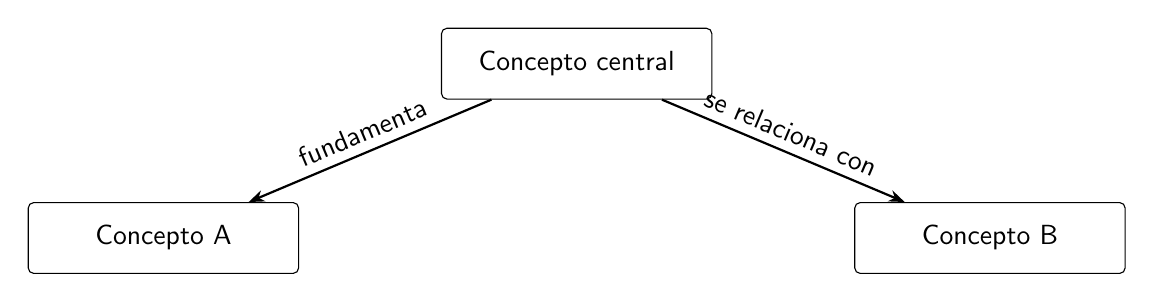
\begin{tikzpicture}[
  concepto/.style={rectangle, draw, rounded corners=2pt,
    align=center, text width=3.2cm, minimum height=0.9cm},
  flecha/.style={-{Stealth[length=2mm]}, thick}
]
\node[concepto] (a) {Concepto central};
\node[concepto, below left=1.3cm and 1.8cm of a] (b) {Concepto A};
\node[concepto, below right=1.3cm and 1.8cm of a] (c) {Concepto B};
\draw[flecha] (a) -- node[above, sloped]{fundamenta} (b);
\draw[flecha] (a) -- node[above, sloped]{se relaciona con} (c);
\end{tikzpicture}
\caption{Mapa conceptual de [tema]}
\end{figure}
\end{verbatim}

\subsubsection*{Línea de tiempo}

\begin{verbatim}
\begin{figure}[H]
\centering
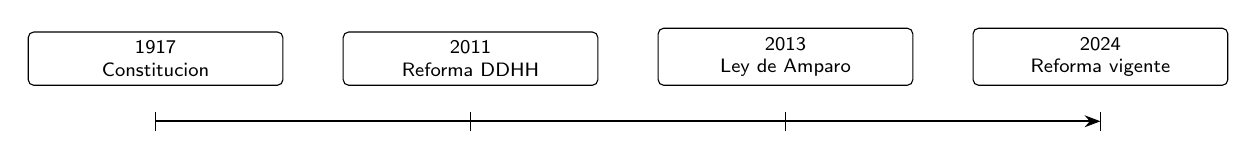
\begin{tikzpicture}[
  evento/.style={rectangle, draw, rounded corners=2pt,
    align=center, text width=3cm, font=\scriptsize},
  eje/.style={-{Stealth[length=2mm]}, thick}
]
\draw[eje] (0,0) -- (12,0);
\foreach \x/\anio/\texto in {
  0/1917/Constitucion,
  4/2011/Reforma DDHH,
  8/2013/Ley de Amparo,
  12/2024/Reforma vigente}
{
  \draw (\x,0.12) -- (\x,-0.12);
  \node[evento, above=0.45cm] at (\x,0) {\anio\\\texto};
}
\end{tikzpicture}
\caption{Linea de tiempo de [tema]}
\end{figure}
\end{verbatim}

\subsubsection*{Diagrama de flujo}

\begin{verbatim}
\begin{figure}[H]
\centering
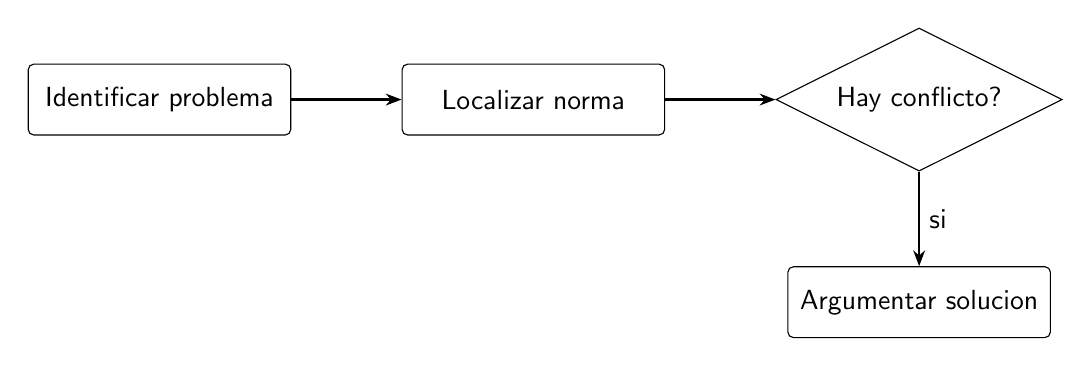
\begin{tikzpicture}[
  paso/.style={rectangle, draw, rounded corners=2pt,
    align=center, text width=3.1cm, minimum height=0.9cm},
  decision/.style={diamond, draw, aspect=2, align=center,
    text width=2.8cm, inner sep=1pt},
  flecha/.style={-{Stealth[length=2mm]}, thick}
]
\node[paso] (inicio) {Identificar problema};
\node[paso, right=1.4cm of inicio] (norma) {Localizar norma};
\node[decision, right=1.4cm of norma] (decision) {Hay conflicto?};
\node[paso, below=1.2cm of decision] (analisis) {Argumentar solucion};
\draw[flecha] (inicio) -- (norma);
\draw[flecha] (norma) -- (decision);
\draw[flecha] (decision) -- node[right]{si} (analisis);
\end{tikzpicture}
\caption{Diagrama de flujo de [proceso]}
\end{figure}
\end{verbatim}

\subsection{Cierre operativo}

La elección de una técnica no debe ser decorativa. Si la actividad pide un producto, la técnica funciona como una herramienta de análisis. El criterio de calidad es que el producto permita ver una decisión intelectual: qué se seleccionó, cómo se organizó, qué relación se construyó y qué postura se puede defender a partir de esa organización.


% BLOQUE OPCIONAL: CUADRO O TABLA AMPLIA
% \clearpage
% \pagestyle{empty}
% \begin{landscape}
% \begingroup
% \scriptsize
% \setlength{\tabcolsep}{4pt}
% \renewcommand{\arraystretch}{1.35}
% \begin{longtable}{@{}p{0.18\linewidth}p{0.39\linewidth}p{0.39\linewidth}@{}}
% \caption{Titulo del cuadro comparativo}\label{tab:cuadro-comparativo}\\
% \toprule
% \textbf{Criterio} & \textbf{Elemento 1} & \textbf{Elemento 2} \\
% \midrule
% \endfirsthead
% \toprule
% \textbf{Criterio} & \textbf{Elemento 1} & \textbf{Elemento 2} \\
% \midrule
% \endhead
% Concepto & \textit{Refuerzo Ciclo A: Contenido sintetico con cita si aplica.} & \textit{Refuerzo Ciclo A: Contenido sintetico con cita si aplica.} \\
% Funcion & \textit{Refuerzo Ciclo A: Contenido.} & \textit{Refuerzo Ciclo A: Contenido.} \\
% Consecuencia & \textit{Refuerzo Ciclo A: Contenido.} & \textit{Refuerzo Ciclo A: Contenido.} \\
% \bottomrule
% \end{longtable}
% \endgroup
% \end{landscape}
% \pagestyle{fancy}

% BLOQUE OPCIONAL: PRODUCTO VISUAL EN TIKZ
% \begin{figure}[H]
% \centering
% \begin{tikzpicture}[
%   node distance=1.3cm,
%   box/.style={rectangle, rounded corners=2pt, draw=black!65, fill=black!4, align=center, minimum width=3.2cm, minimum height=0.9cm},
%   arrow/.style={-{Latex[length=2.5mm]}, thick, draw=black!65}
% ]
%   \node[box] (centro) {Concepto central};
%   \node[box, right=of centro] (relacion) {Concepto relacionado};
%   \node[box, below=of relacion] (efecto) {Consecuencia};
%   \draw[arrow] (centro) -- node[above]{implica} (relacion);
%   \draw[arrow] (relacion) -- node[right]{produce} (efecto);
% \end{tikzpicture}
% \caption{Titulo del producto visual.}
% \end{figure}

% SECCION 4: POSTURA PERSONAL

\section{Postura personal}

\textit{Refuerzo Ciclo A: Redactar una postura academica y moderada. Formula util: posicion, razon y efecto.}

% SECCION 5: CONCLUSION

% --- Ciclo A: refuerzo editorial materializado ---
\section*{Refuerzo editorial Ciclo A}
Este apartado consolida la mejora editorial incremental del nodo a partir del estándar maduro de AulaTeX. El refuerzo atiende brechas detectadas de bibliografía, citas, análisis propio, transferencia y cierre argumentado, sin sustituir la consigna original ni copiar contenido de los casos maestros.

\subsection*{Tesis de trabajo}
La actividad debe sostener una postura verificable: el producto solicitado no sólo organiza información, sino que permite interpretar el problema disciplinar, justificar decisiones y reconocer sus consecuencias académicas o profesionales.

\subsection*{Análisis propio}
El hallazgo central es que una entrega madura requiere pasar de la descripción a la interpretación. Por ello, el desarrollo debe explicar qué revela el producto construido, por qué es relevante para la materia y qué criterio permite evaluar su pertinencia. Esta operación convierte la evidencia reunida en argumento académico.

\subsection*{Transferencia profesional}
La transferencia consiste en vincular el producto con situaciones reales de desempeño: diagnóstico, toma de decisiones, comunicación de resultados, cumplimiento normativo, intervención educativa o resolución de problemas según el campo disciplinar. Así, la actividad adquiere valor formativo más allá de la plantilla.

\subsection*{Cierre argumentado}
En consecuencia, la calidad de la actividad depende de que el producto visible, las fuentes y la conclusión formen una secuencia coherente. La conclusión debe recuperar la tesis, indicar el principal aprendizaje y señalar una implicación práctica o conceptual.

% Brechas locales atendidas por Ciclo A: analisis_propio, conclusion_argumentada, bibliografia_insuficiente, citas_insuficientes, pendientes_editoriales
% Reglas globales aplicadas:
% - Priorizar cierre de brecha recurrente: bibliografia_insuficiente (427 nodos).
% - Priorizar cierre de brecha recurrente: conclusion_argumentada (375 nodos).
% - Priorizar cierre de brecha recurrente: citas_insuficientes (328 nodos).
% - Priorizar cierre de brecha recurrente: analisis_propio (288 nodos).
% --- Fin Ciclo A ---

\section{Conclusion}

% REFLEXION PERSONAL:
% Sintetizar aprendizaje, postura final, transferencia y mejora futura.

\textit{Refuerzo Ciclo A: Cerrar con sintesis, aprendizaje, implicacion y criterio final. No introducir informacion nueva.}

\clearpage
\nocite{itescaSitioWeb,itescaMGAOferta,inegiPIBE2024,inegiPIBActividad,conevalPobrezaMexico,economiaDataMexicoSonora}
\bibliography{\itescabibliography}






































































































\subsection*{Citas de refuerzo Ciclo A}
La mejora editorial se vincula con la memoria documental disponible mediante las referencias \citep{itescaMGAOferta,inegiPIBE2024,inegiPIBActividad,conevalPobrezaMexico}. Estas citas deben revisarse en una etapa disciplinar fina para sustituir o complementar fuentes genéricas por literatura específica del tema.

\end{document}






